\section{Illustrative Examples}
\label{}

\begin{figure}[htbp]
\centering
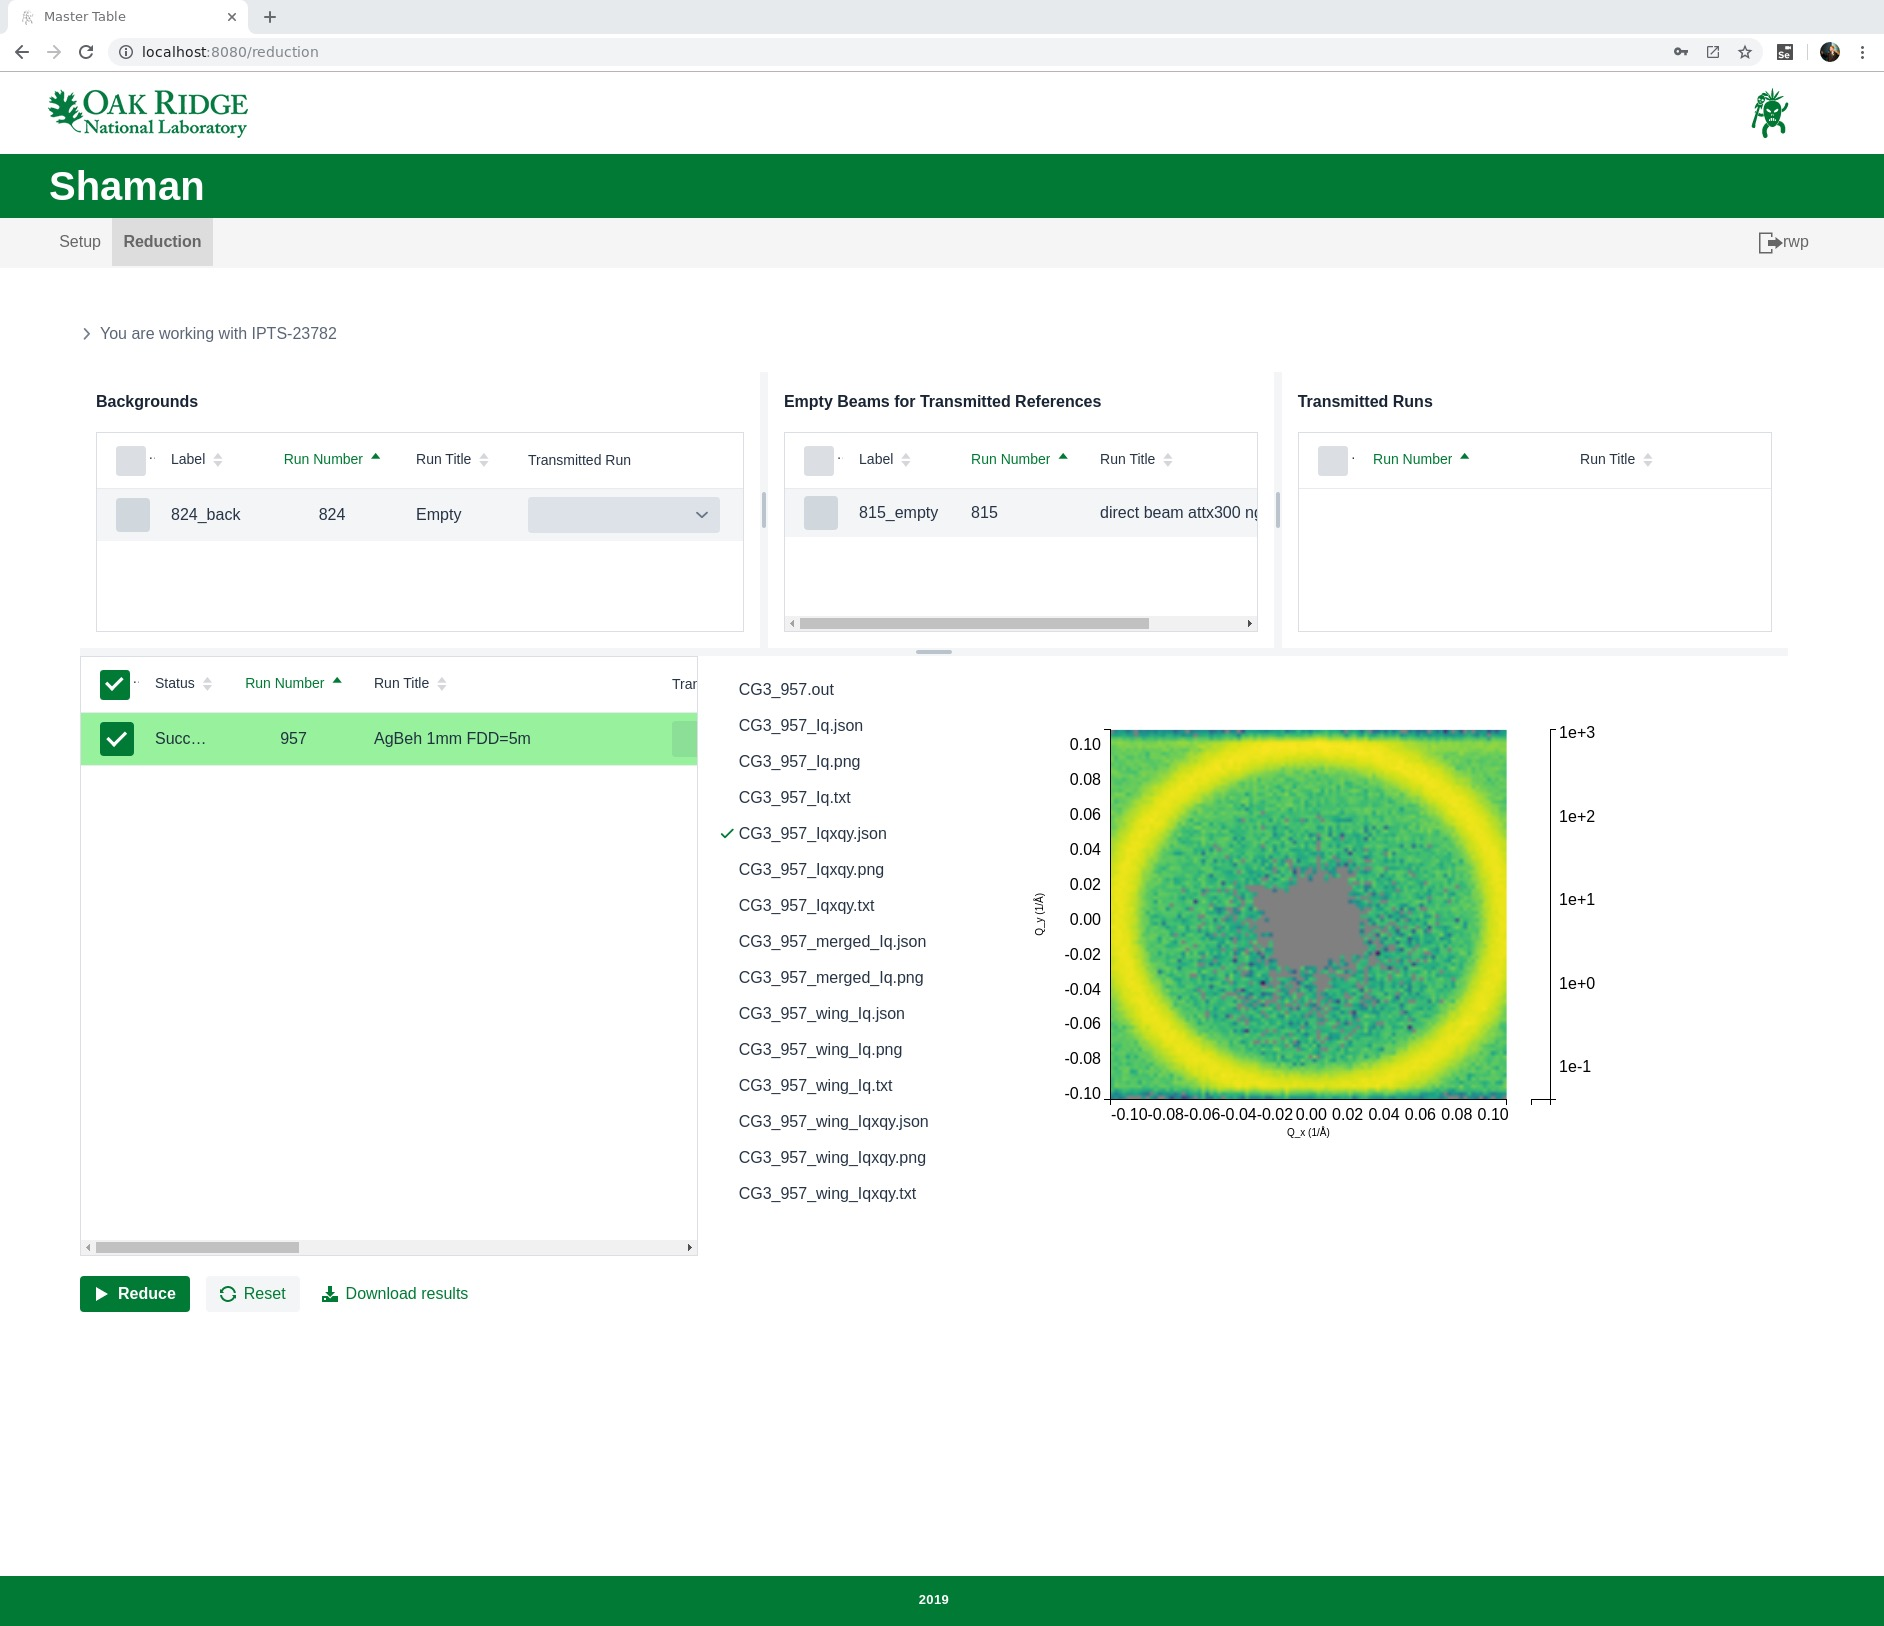
\includegraphics[width=\textwidth]{shaman-paper-2019/src/figures/biosans-IQXY.jpg}
\caption{The 2D intensity as a function of wave vector in the main BIOSANS detector as shown in Shaman.}
\label{biosans-main}
\end{figure}

\begin{figure}[htbp]
\centering
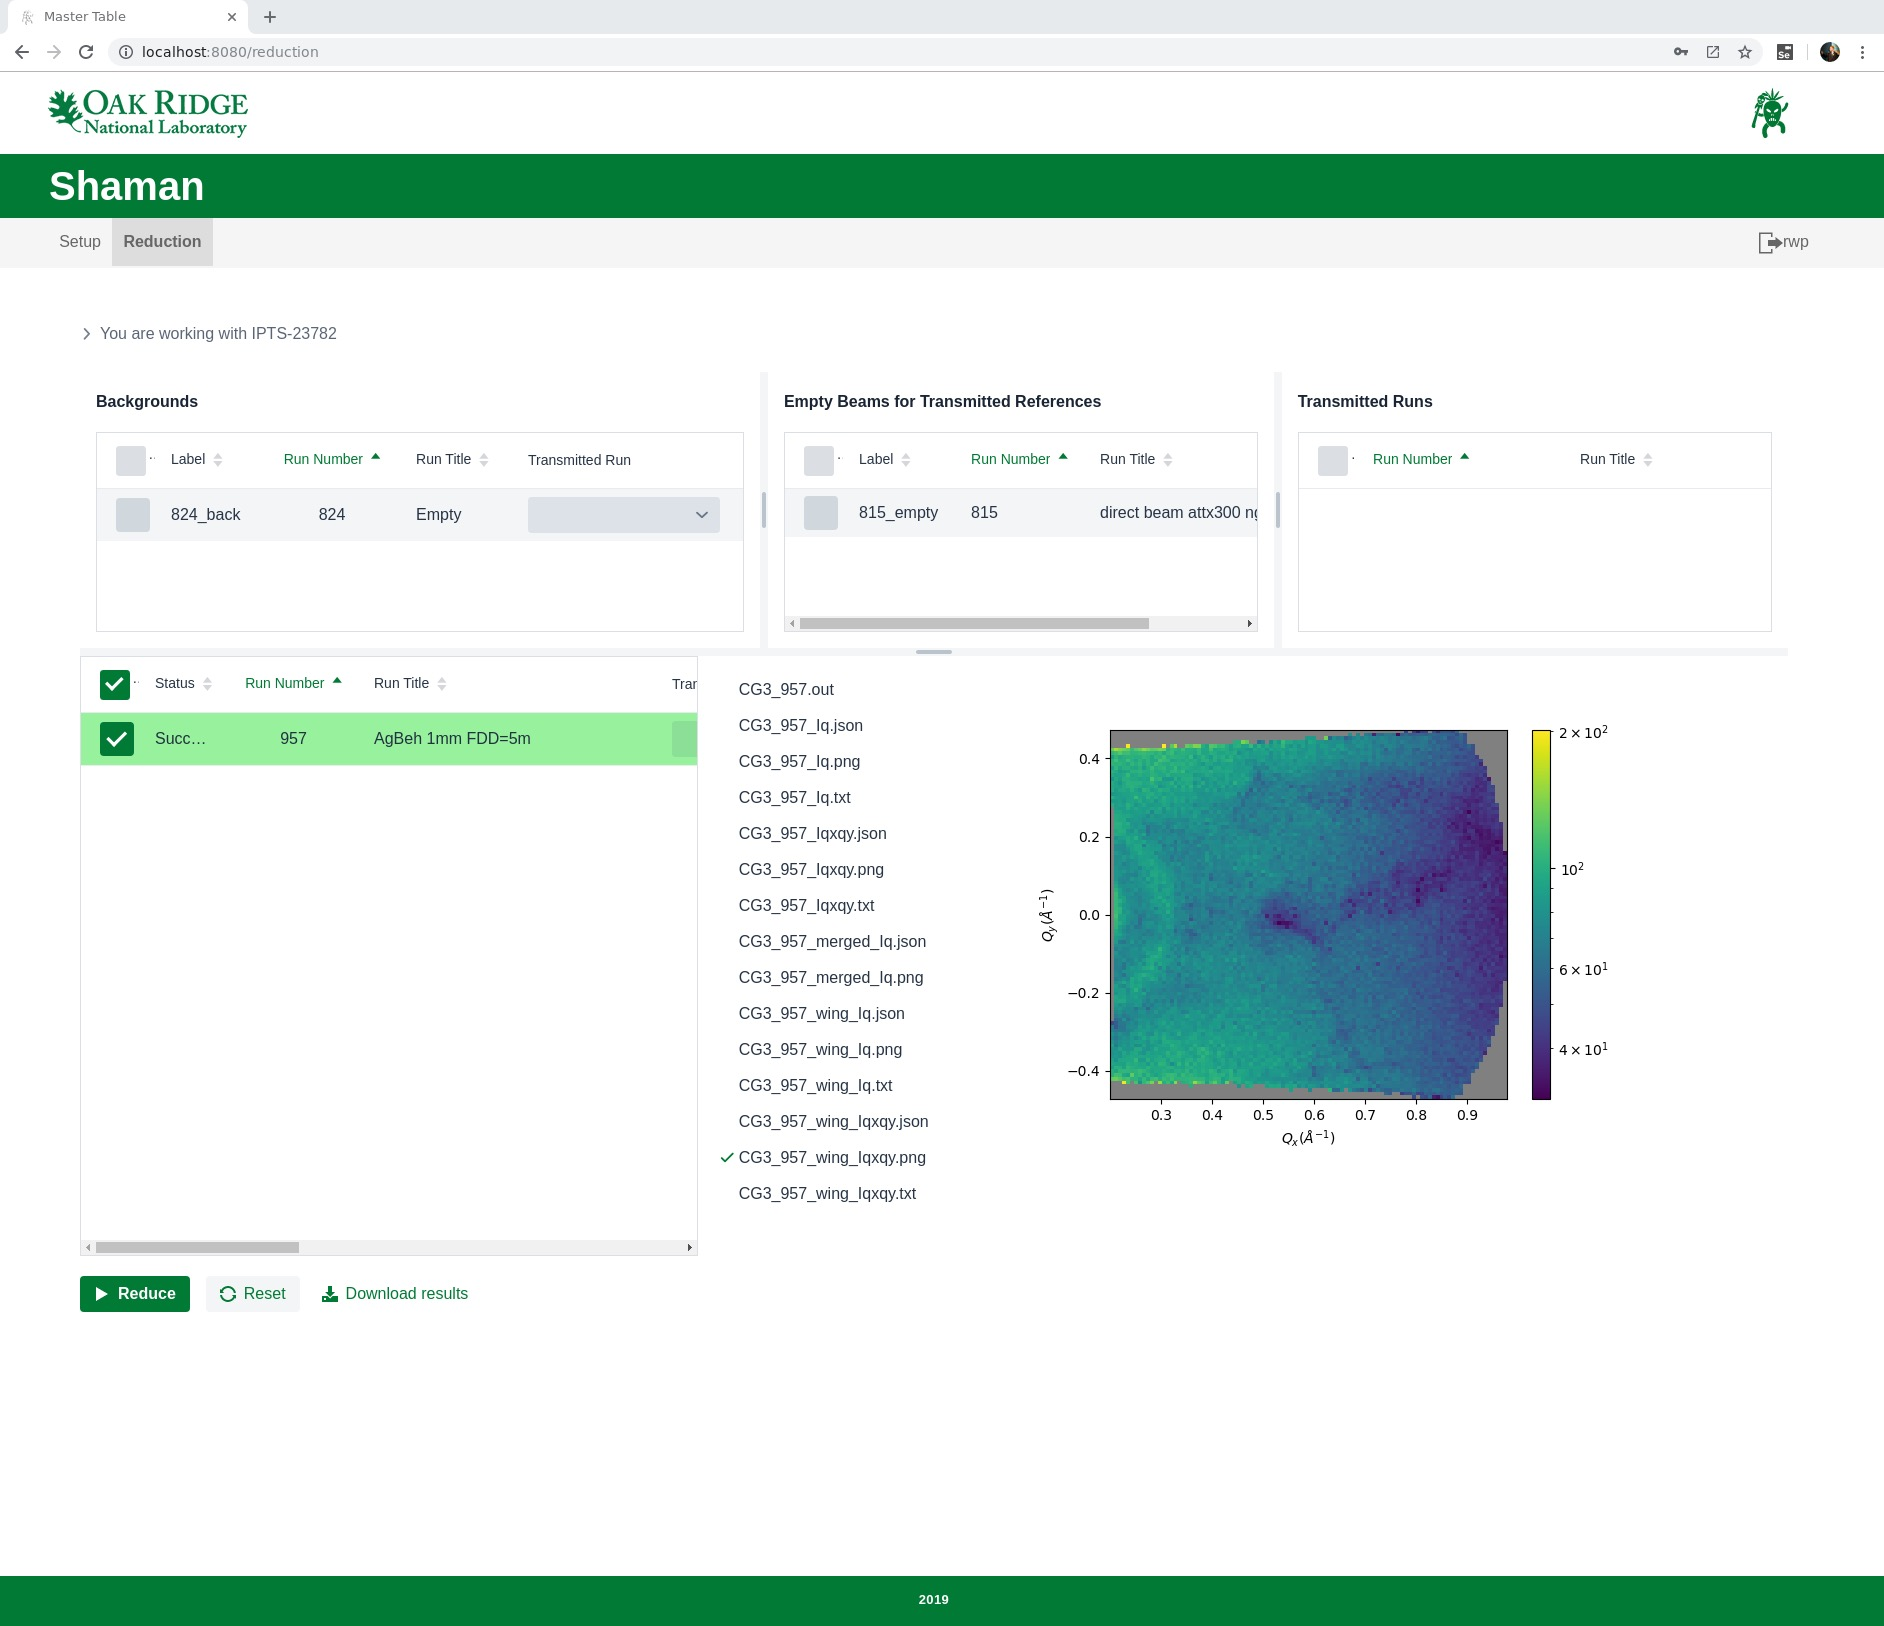
\includegraphics[width=\textwidth]{shaman-paper-2019/src/figures/biosans-IQ-wing.jpg}
\caption{The 2D intensity as a function of wave vector in the BIOSANS wing detector as shown in Shaman.}
\label{biosans-wing}
\end{figure}


Provide at least one illustrative example to demonstrate the major functions.

Optional: you may include one explanatory video that will appear next to your article, in the right hand side panel. (Please upload any video as a single supplementary file with your article. Only one MP4 formatted, with 50MB maximum size, video is possible per article. Recommended video dimensions are 640 x 480 at a maximum of 30 frames/second. Prior to submission please test and validate your .mp4 file at $ http://elsevier-apps.sciverse.com/GadgetVideoPodcastPlayerWeb/verification$. This tool will display your video exactly in the same way as it will appear on ScienceDirect.).